\documentclass[11pt,twocolumn]{article}

\usepackage{array}
\usepackage{clrscode3e}
\usepackage{amsmath}
\usepackage{kbordermatrix}
\usepackage{mathtools}
\usepackage{cite}
\usepackage{hyperref}
\usepackage{rotating}
\usepackage{pdfpages}

\newcommand{\defeq}{\vcentcolon=}
\newcommand{\eqdef}{=\vcentcolon}

\setlength{\parindent}{0em}
\setlength{\parskip}{1em}

\begin{document}

\title{Efficient Calculation of Polynomial and Interaction Features on Sparse Matrices}
\author{
  Andrew Nystrom\\
  \texttt{awnystrom@gmail.com}
  \and
  John Hughes\\
  \texttt{jfh@cs.brown.edu}
}
\date{}

\maketitle

\begin{abstract}%   <- trailing '%' for backward compatibility of .sty file
We give an algorithm to efficiently calculate second degree polynomial or interaction features for a sparse matrix.
The algorithm has average time complexity that decreases quadratically with respect to the density of the matrix, which
is a large improvement over the naive approach. It also allows for the matrix to remain in sparse form, reducing memory demands.
We apply the method to several real datasets and give both analytical and empirical comparisons with the
naive approach. The work also gives a generalizable method for creating algorithms for higher orders of polynomials.
\end{abstract}

\section{Introduction}

When performing a modeling task, one is often faced with a non-linearly separable problem,
or is attempting to predict a target that is a non-linear combination of the variables at one's disposal.
There are several general classes of methods for dealing with these situations: kernel methods, 
high variance models, and input transformations.

Of the possible types of input transformations one
might apply, a widely used method is the polynomial transformation, which is defined as 
all products of all combinations with replacement of $k$ components of a $D$ dimensional row vector $\vec{x}$ (assuming row-wise instance representation), where $k$ is the degree of the polynomial.
In the case of $k=2$, the following set of polynomial features are augmented to each $\vec{x}_i$:

\begin{equation*}
\{x_a \cdot x_b : a, b \in \{0,1,..., D-1\} \land a \le b\}
\end{equation*}

which results in $\binom{D+1}{D-1} = \frac{D^2+D}{2}$ additional features, so the generation of 
these features for a matrix of size $N \times D$ has a time complexity of $O(ND^2)$. In the general case of degree $k$, there 
are $\binom{D+k-1}{D-1}$ polynomial features and the time complexity is $O(ND^k)$.

To show the types of nonlinearity polynomial features are capable of imbuing a linear model with,
we trained logistic regression models on four inseparable datasets and plot their decision boundaries, as seen in figure \eqref{fig:boundaries} on page \pageref{fig:boundaries}. We compare
these decision boundaries to those learnt by more complex methods, namely a support vector machine with a radial basis function kernel\footnote{\url{http://scikit-learn.org/stable/modules/generated/sklearn.svm.SVC.html}} 
and gradient boosted decision trees\footnote{\url{https://github.com/dmlc/xgboost/}}. As can be seen, polynomial features allow a simple linear classifier is capable of drawing decision boundaries
that in the form of arbitrary parabolas, hyperbolas, and elipses.

Beyond classification, polynomial regression \cite{theoryoflinearmodels} is a staple regression method.
We provide a demonstration of the power polynomial features can lend to a regression problem by fitting two ordinary least squares models to $y=sin(x) + \mathcal{N}(0, 0.1), x \in [0, \pi]$. The first model (the blue curve) was given only $x$ as its input. The second model (the green curve) was given $x$ and second degree polynomial features derived from $x$ (namely $x^2$). The curves the models learned can be seen in figure \ref{fig:regression}.

While polynomial features are a well known and used concept in machine learning (e.g. \cite{pavlidis2002learning, konidaris2009skill, wiesler2009investigations}) and work has been done to improve their utilization (e.g. \cite{pevckov2008minimal, huang2010predicting}), this is the first work that we know of that exploits matrix sparcity 
to improve the speed with which they are calculated and allows them to be calculated for a sparse matrix.


\begin{sidewaysfigure}
    \centering
    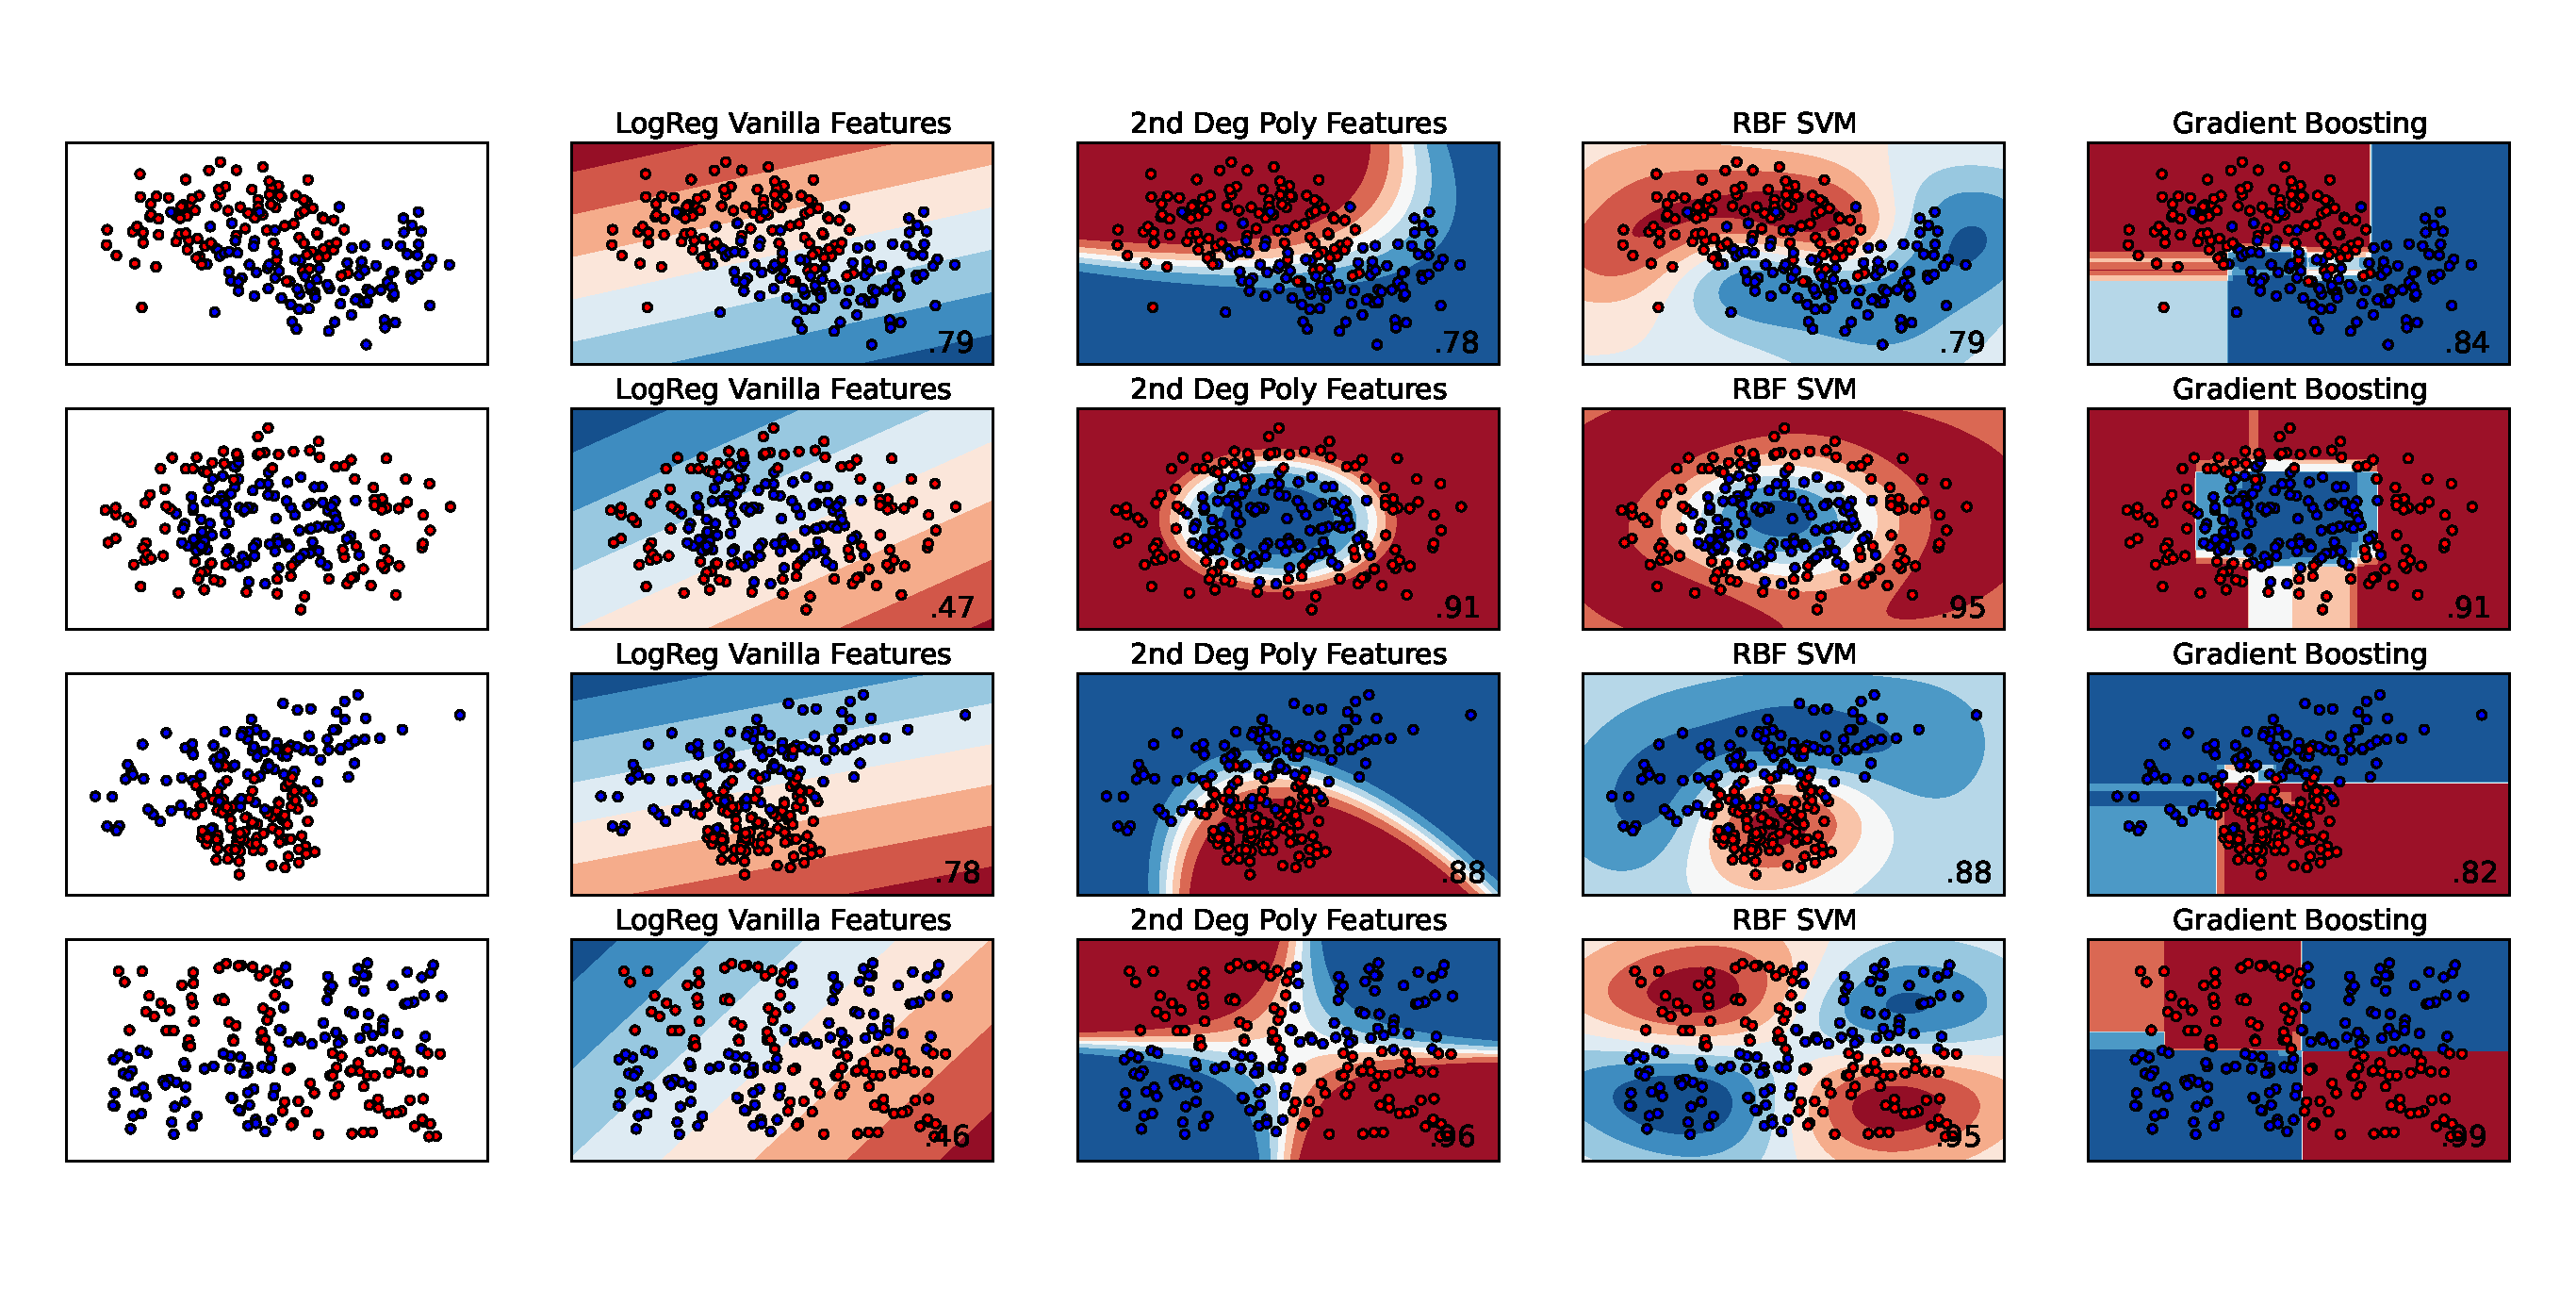
\includegraphics[scale=0.25]{boundaries.eps}
    
     \caption{\footnotesize{Decision boundaries for four classifier types on four different datasets. The darker the color, the more certain the decision.
             The plain dataset is shown in the first column. Each other column is a type of classifier applied to that dataset. The classifier
             types are logistic regression, logistic regression with second degree polynomial features, RBF SVM, and gradient boosting with decision trees.
             The accuracy of each model is shown in the bottom right corner of that model's subplot.}}
    \label{fig:boundaries}
\end{sidewaysfigure}

\begin{figure}
    \centering
    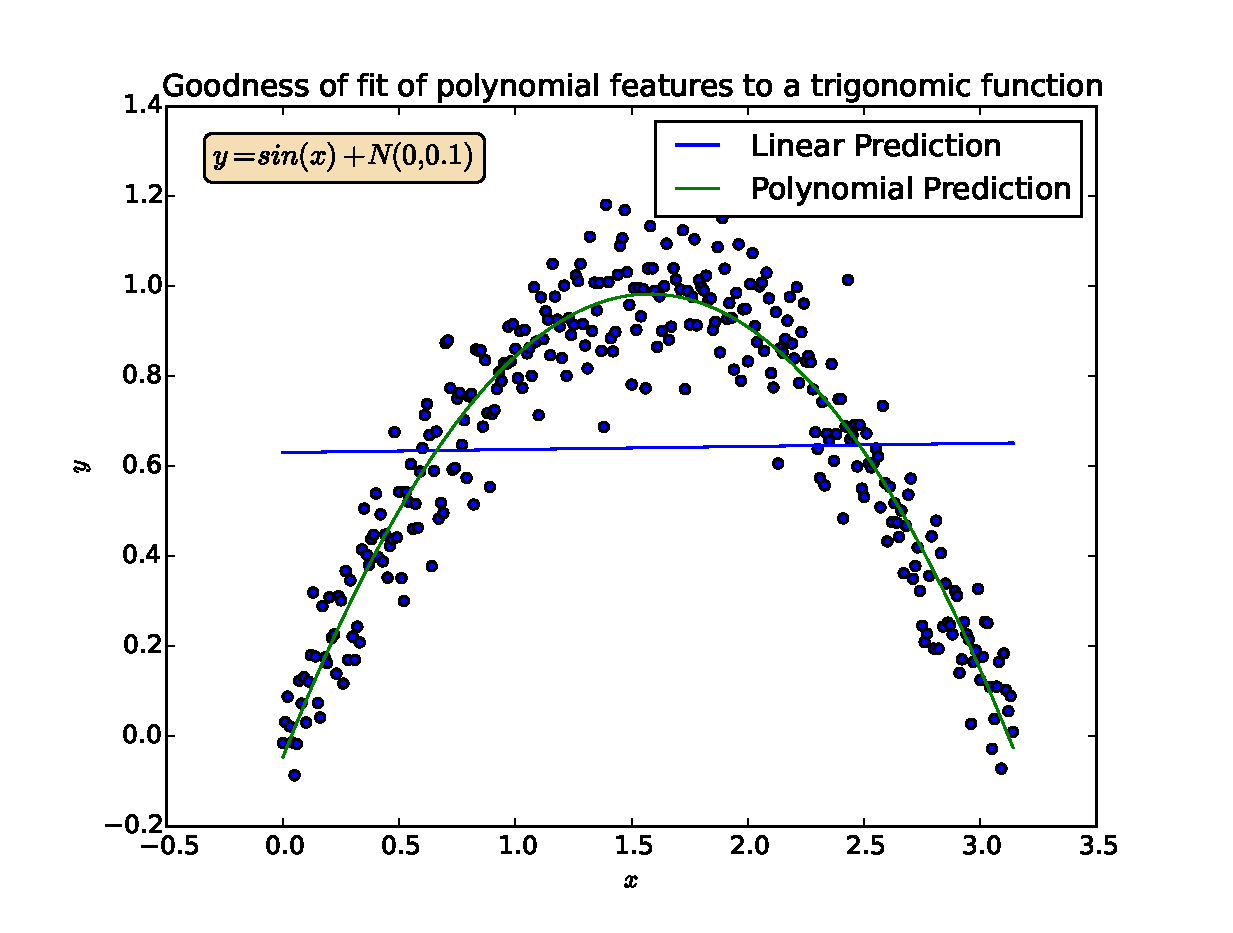
\includegraphics[scale=0.4]{regression.eps}
     \caption{\footnotesize{Two linear regression models fit to $y=sin(x) + \mathcal{N}(0, 0.1), x \in [0, \pi]$. The blue line's model was given only $x$, while the green line's model was given $x$ and second degree polynomial features.}}
    \label{fig:regression}
\end{figure}

%\newpage


\section{Sparse Polynomial Features} \label{sec:sparse}
If the vectors of a feature matrix are sparse, many of these products of features will be
zero, and are therefore unnecessary to calculate if the matrix is stored in a sparse matrix 
data structure. If the density (the fraction of nonzero elements) of the matrix is $d$ where $0 \le d \le 1$,
the number of nonzero polynomial features is

\begin{equation*}
\binom{dD+2-1}{dD-1} = \frac{d^2D^2+dD}{2}
\end{equation*}

and if only they were calculated, the time complexity of generating polynomial features
for a matrix of size $N \times D$ is $O(Nd^2D^2)$, quadratically lower than calculating them via brute force.

The question then is how to devise an algorithm to calculate polynomial features for a vector $\vec{x}$ so that
only the nonzero elements of $\vec{x}$ are considered during the calculation process. Two main components are needed: (1) the ability to
quickly access only the nonzero elements of $\vec{x}$ and (2) The ability to know which polynomial feature column
the product of features with indices $a$ and $b$ should be stored in.

The first of these necessary components is obtained simply by using the appropriate data structure
to store the sparse matrix (e.g. storing it in compressed sparse row form). The second component 
is not only less readily available, but its necessity is less obvious. To make this need more clear, consider the
algorithm for the brute force calculation of polynomial features:

\begin{codebox}
\footnotesize
\Procname{$\proc{Dense Polynomial Features}(A)$}
    \zi $N \gets$ row count of $A$
    \zi $D \gets$ column count of $A$
    \zi $B$ $\gets$ Matrix of size $N \times \frac{D^2+D}{2}$
    \zi \For $\id{row}$ in $A$ \Do
    \zi     $k \gets 0$
    \zi     \For $\i \gets 0 \To D$ \Do
    \zi         \For $\j \gets i \To D$ \Do
    \zi             $r \gets$ index of $\id{row}$
    \zi             $B[r, k] \gets \id{row}[i] \cdot \id{row}[j]$
    \zi             $k \gets k + 1$
                \End
            \End
       	\End
\end{codebox}

Notice that, for an individual row, the location of a polynomial feature ($\id{row}[i] \cdot \id{row}[j]$) can be determined
by a simple counter $k$ that is incremented each pass through the inner loop. This cannot be
done if we only calculate products between nonzero elements of $\vec{x}$, because all that
will be known is the nonzero element indices - many iterations will be skipped (hence the improved computational complexity).

What is therefore needed is a mapping between row-column index pairs of $\vec{x}$ and the space ${0, 1, ..., \frac{D^2+D}{2}-1}$
(the output size of second degree polynomial features when $D = |\vec{x}|$). The ordering of the mapping is irrelevant so long as its input 

\begin{equation*} \label{eq:input}
I \defeq \{(a, b) : a, b \in \{0,1,..., D-1\} \land a \le b\}
\end{equation*}

is bijective with its output

\begin{equation*} \label{eq:output}
O \defeq \{0, 1, ..., \frac{D^2+D}{2}-1\}
\end{equation*}


Interaction features are a way of capturing correlations between features in a machine 
learning setting. A feature vector $\vec{x}$ of dimensionality $D$ has second degree interaction features 
$\{x_i \cdot x_j : i, j \in \{0,1,..., D-1\} \land i < j\}$, 
so a $D$ dimensional vector has $\binom{D}{2} = \frac{D^2-D}{2}$ second degree interaction features. A naive
approach to calculating these features is to simply iterate through the combinations of the column indices.
For a sparse vector, many of the resulting interaction features would be zero, and could therefore be ignored.
This work describes a method to efficiently calculate second degree interaction features for a sparse matrix 
that has time and space complexities that decrease quadratically with the density of the input matrix with respect to the naive approach.

\section{Approach}
Let the list of nonzero columns for a given row $\vec{x}$ be denoted by $N_{zc}$. The nonzero second degree 
interaction features are simply the products of all combinations of two elements whose 
columns are in $N_{zc}$. However, to properly place an interaction feature into the correct column, a mapping from the column 
index pairs of $N_{zc}$ into the columns of the interaction matrix is needed. The mapping is 
from pairs $(i, j)$,  where $i$ and $j$ are in $0, 1, \ldots , D-1$, and $i < j$, to $0, 1,2,..., \frac{D^2-D}{2} - 1$,  Such a mapping essentially consists of mapping the indices of entries in the upper triangle of a matrix to indices in a flat 
list. We now describe the construction of such a mapping. 

\subsection{Mapping construction}

We seek a map from matrix indices $(i, j)$ (with $i < j$ and $0 \le i < D$) to numbers $f(i, j)$ with $0 \le f(i, j) < \frac{D(D-1)}{2}$, one that follows the pattern indicated by 
\begin{align}
\begin{bmatrix}
x & 0 & 1 & 3 \\
x & x & 2 & 4 \\
x & x & x & 5 \\
x & x & x & x
\end{bmatrix}
\label{eq:4x4mat}
\end{align}
where the entry in row $i$, column $j$, displays the value $f(i, j)$. 

To simplify slightly, we introduce a notation for the $n$th triangular number, 
\begin{align}
T_2(n) = \frac{n(n+1)}{2}
\end{align}
\noindent
The subscript $2$ indicates that these are triangles in two dimensions; we'll use $T_3(n)$ to indicate the $n$th tetrahedral number, and so on for higher dimensions. 

Observe that in Equation~\ref{eq:4x4mat}, each entry in column $j$ (for $j > 0$) lies in the range
\begin{align}
T_2(j-1) &\le e < T_2(j).
\end{align}
\noindent
And in fact, the entry in the $i$th row of that column is just $i + T_2(j-1)$. Thus we have
\begin{align}
f(i, j) 
&= i + T_2(j-1)\\
&= i + \frac{(j-1)j}{2}\\
&=  \frac{2i + j^2-j}{2}.
\end{align}

For instance, in column $j = 2$ in our example (the \emph{third} column), the entries range from $1$ to $2$, while $T_2(j-1) = T_2(1) = 1$ and $T_2(j) = T_2(2) = 3$, and the entry in column $j = 2$, row $i = 1$ is 
$i + T_2(j-1) = 1 + 1 = 2$. 

\subsubsection{Other indices}
With one-based indexing in both the domain and codomain, the formula above becomes
\begin{align}
f_1(i, j) &= 1+ f(i-1, j-1) \\
&= 1+ f(i-1, j-1) \\
& = \frac{2 + 2(i-1) + (j-1)^2-(j-1)}{2}\\
& = \frac{2i + j^2 - 3j + 2}{2}
\end{align}

\subsubsection{Polynomial Features}
For polynommial features, we seek a map from matrix indices $(i, j)$ (with $i \le j$ and $0 \le i < D$) to numbers $g(i, j)$ with $0 \le f(i, j) < \frac{D(D+1)}{2}$, one that follows the pattern indicated by 
\begin{align}
\begin{bmatrix}
 0 & 1 & 3 & 6 \\
 x & 2 & 4 & 7\\
 x & x & 5 & 8 \\
 x & x & x & 9
\end{bmatrix}
\label{eq:4x4mat-poly}
\end{align}
i.e., essentially the same task as before, except that the diagonal is included. One can regard all but the last column of entries in Equation~\ref{eq:4x4mat-poly} as corresponding to the entries in Equation~\ref{eq:4x4mat}, but shifted to the left. Thus the formula for $g(i, j)$ is simply the formula for $f$, shifted by 1, i.e., 
\begin{align}
g(i, j) &= f(i, j+1)  \\
&=  \frac{2i + (j+1)^2-(j+1)}{2}\\
&=  \frac{2i + j^2 + j + 1)}{2}.
\end{align}
Alternatively, we can write this as
\begin{align}
g(i, j) &= i + T_2(j),
\end{align}
\noindent
and get the same result. 


\subsubsection{Higher dimensions}
To handle three-way interactions, we need to map triples of indices in a 3-index array to a flat list, and similarly for higher-order interactions. 

For three indices, $i,j,k$, with $i < j < k$ and $0 \le i,j,k < D$, we have a similar recurrence. Calling the mapping $h$, we have 
\begin{align}
h(i,j,k) = i + T_2(j-1) + T_3(k-2);
\end{align}
if we define $T_1(i) = i$, then this has the very regular form
\begin{align}
h(i,j,k) =  T_1(i) + T_2(j-1) + T_3(k-2);
\end{align}
and from this, the generalization to higher dimensions is straightforward. The formulas for ``higher triangular numbers'', i.e., those defined by
\begin{align}
T_k(n) &= \sum_{i=1}^n T_{k-1}(n)
\end{align}
for $k > 1$ can be determined inductively. For $k = 3$, the result is 
\begin{align}
T_3(n) &= \sum_{i=1}^n T_{2}(n)\\
&= \frac{n^3 + 3n^2 + 2n}{6},
\end{align}
so that the formula for 3-way interactions, with zero-based indexing, becomes 
\begin{align}
h(i, j, k) &= 1 + (i-1) + \frac{(j-1)j}{2} + \\
& \frac{(k-2)^3 + 3(k-2)^2 + 2(k-2)}{6}. 
\end{align}
\subsubsection{Higher-dimension polynomial features}
For the case where we include the diagonal in higher dimensions, we must shift $j$ by $1$, $k$ by $2$, and so on, and the formula becomes
\begin{align}
\ell(i,j,k) =  T_1(i) + T_2(j) + T_3(k),
\end{align}
with analogous formulas for higher degree polynomial interactions. 

\subsection{Inversion}
We not only want to be able to compute the ``flat index'' $f(i,j)$ corresponding to a particular index pair $(i, j)$, we'd like, given a value $N = f(i, j)$, to be able to determine $i$ and $j$. We know, given $N$, that $f(0, j) \le N \le f(j,j-1)$, i.e., that 
\begin{align}
\frac{j^2 - 3j + 2}{2} &\le N \le \frac{2(j-1) + j^2 - 3j + 2}{2}\\
{j^2 - 3j + 2} &\le 2N \le {j^2 - j}.
\end{align}
If we find the (real number) value $j_{*}$ for which $j_{*}^2 - j_{*} = 2N$, then we know that $j = \lfloor j_{*}\rfloor$. Finding $j_{*}$ amounts to solving a quadratic, whence
\begin{align}
j_{*} = \frac{1 \pm \sqrt{1 + 8N}}{2}.
\end{align}
Clearly the larger value, 
\begin{align}
j_{*} = \frac{1 + \sqrt{1 + 8N}}{2},
\end{align}
is the one we seek; we set $j = \lfloor j_{*}\rfloor$, and compute $i = N - \frac{j^2 - j}{2}$. 
In practice, repeatedly computing square roots may be annoying; instead, when we compute $N = f(i,j)$, we can record the values of $i$ and $j$ along with the interaction features, making inversion a simple matter of looking up these values. 


Similarly, for polynomial features, to invert 
\begin{align}
g(i, j) &=  \frac{2i + j^2 + j + 1)}{2}
\end{align}
we know that if $N = g(i,j)$, then $g(0,j) \le N \le g(j,j)$, which tells us that 
\begin{align}
2N \le j^2 + 3j + 1, \text{ so}\\
0 \le j^2 + 3j + (1-N^2)
\end{align}. 
Solving for $j$ when this last inequality is an equality, we get 
\begin{align}
j_{*} = \frac{-3 \pm \sqrt{ 5 - N^2 }}{2}; 
\end{align}
Once again, we set $j = \lfloor j_{*}\rfloor$, and compute $i = N - \frac{j^2 + j + 1}{2}$. 

Inverting the higher-order formulas, which involve cubics, quartics, etc., is infeasible, but storing the inverse map as described above may be practical, especially for sparse feature sets. 

\section{The Algorithm}
In section X we showed why a mapping from the space X
onto the space X is necessary for calculating polynomial features for a sparse matrix, then
derived such a mapping.

We now have the necessary components for an algorithm to efficiently calculate polynomial features for
a sparse matrix. The matrix needs to be stored in a form that allows for its nonzero column indices, e.g. in sparse row form,
and we will use the mapping derived in X to determine which column in the output space
the polynomial feature between two input columns is mapping onto. Combining these ideas yields the following algorithm:

\begin{codebox}
\footnotesize
\Procname{$\proc{Sparse Polynomial Features}(A)$}
    \zi $\func{PolyMap}(a, b) = \frac{2Da-a^2+2b-3a-2}{2}+a+1$
    \zi $N \gets$ row count of $A$
    \zi $D \gets$ column count of $A$
    \zi $B$ $\gets$ empty sparse $N \times \frac{D^2+D}{2}$ matrix
    \zi \For $\id{row}$ in $A$ \Do
    \zi     $N_{zc} \gets$ nonzero columns of $row$
    \zi     \For $i \gets 0 \To |N_{zc}|$ \Do
    \zi         \For $j \gets i \To |N_{zc}|$ \Do
    \zi             $k \gets \func{PolyMap}(N_{zc}[i], N_{zc}[j])$
    \zi             $r \gets$ index of $\id{row}$
    \zi             $B[r, k] \gets \id{row}[N_{zc}[i]] \cdot \id{row}[N_{zc}[j]]$
                \End
            \End
       	\End
\end{codebox}

Using the mapping for interaction features and changing the bounds in the loop conditions and the size of the output matrix, 
the algorithm can be modified to give second order interaction features:

\begin{codebox}
\footnotesize
\Procname{$\proc{Sparse Interaction Features}(A)$}
    \zi $\func{InterMap}(a, b) = \frac{2Da-a^2+2b-3a-2}{2}$
    \zi $N \gets$ row count of $A$
    \zi $D \gets$ column count of $A$
    \zi $B$ $\gets$ empty sparse $N \times \frac{D^2-D}{2}$ matrix
    \zi \For $\id{row}$ in $A$ \Do
    \zi     $N_{zc} \gets$ nonzero columns of $row$
    \zi     \For $i \gets 0 \To |N_{zc}|-1$ \Do
    \zi         \For $j \gets i+1 \To |N_{zc}|$ \Do
    \zi             $k \gets \func{InterMap}(N_{zc}[i], N_{zc}[j])$
    \zi             $r \gets$ index of $\id{row}$
    \zi             $B[r, k] \gets \id{row}[N_{zc}[i]] \cdot \id{row}[N_{zc}[j]]$
                \End
            \End
       	\End
\end{codebox}

where $N_{zc}$ are the columns of nonzero elements of row $\id{row}$.

\section{Analysis}

\subsection{Analytical}
We assume the input matrix $A$ is in sparse row form. The steps prior to the first loop are
constant operations. The outer loop will be executed $N$ times (once for each row). For each row, 
the innermost loop will be executed and the inner loop will be $\frac{|N_{zc}|^2+|N_{zc}|}{2}$ times.
If the density is uniformly distributed across all rows, $E[|N_{zc}|] = dD$, but this cannot be assumed. In the worst case,
then, the innermost loop will each be executed $\frac{D^2+D}{2}$ times, but on average, $\frac{d^2D^2+dD}{2}$ times.
The operations in the innermost loop are constant. The time complexity is therefore $O(ND^2)$ and $\Theta(Nd^2D^2)$.

In machine learning, an input matrix often has near uniform density across its rows.
For example, if the matrix is sparse due to one-of-m encoding (also known as one-hot vectors), each row vector will
have the same number of nonzero components.

\subsection{Empirical}
To assess the performance of the algorithm on data of varied density, we compare its speed
to the PolynomialFeatures class of the popular machine learning scikit-learn \cite{scikit-learn}.
Uniformly random matrices of size $100 \times D$ were generated for $d=0.1$, $0.2$, $0.3$, $0.4$, and $0.5$, and 
$D=1$, $101$, $201$, $301$, $401$, and $501$. Each point was resampled five times and averaged to decrease variance. Since the scikit-learn version of the algorithm
does not exploit sparsity, we assume the method's time is invariate with respect the density of the matrix, but
we gave it the lowest density of each dimensionality to be fair. The results are shown in figure \eqref{fig:benchmark} on page \pageref{fig:benchmark}.

\begin{figure}[ht, numbered]
    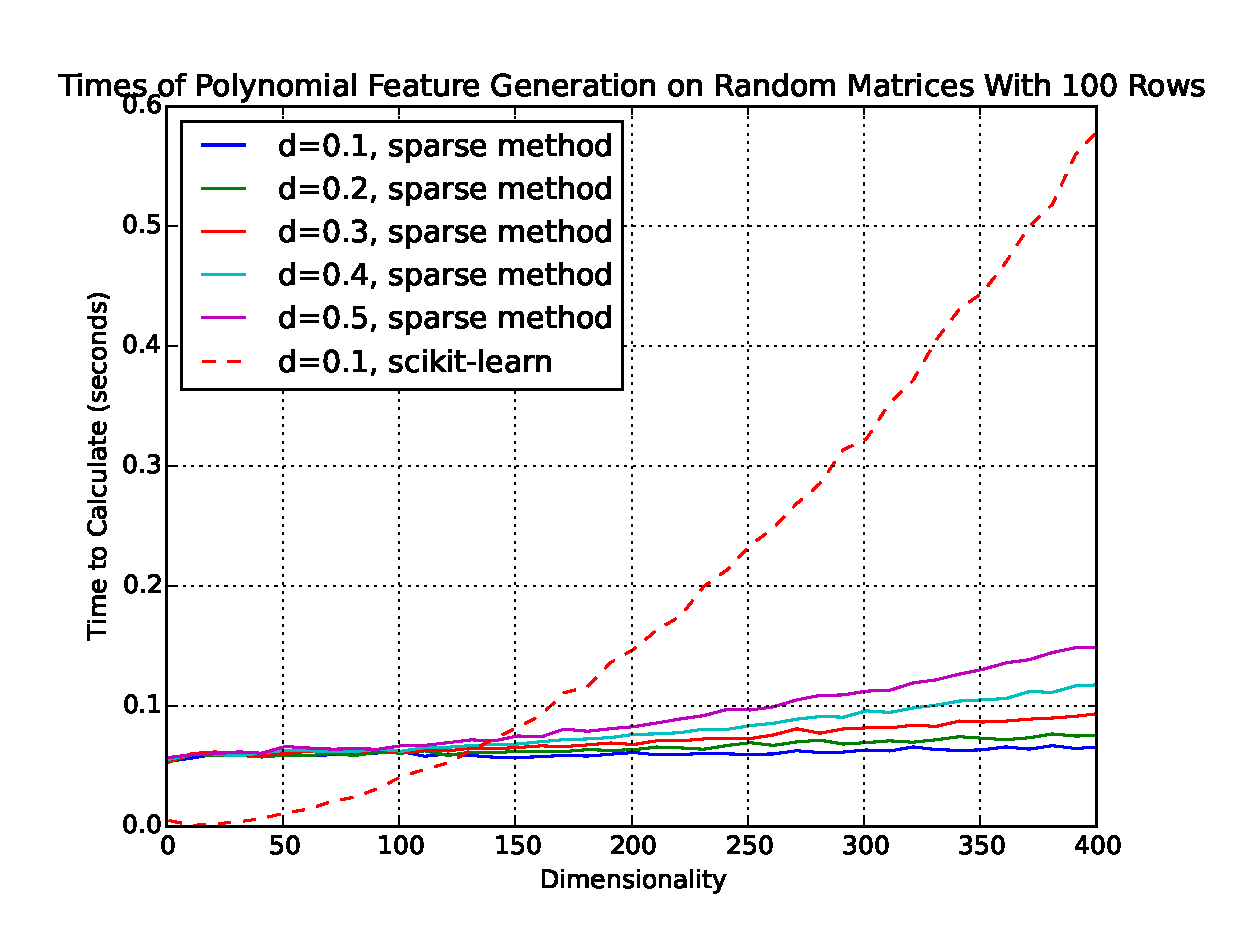
\includegraphics[scale=0.4]{benchmark.eps}
    \caption{This plot shows how long the sparse polynomial method took to run on matrices with 1000 rows of various dimensionalities and densities and compared to the scikit-learn PolynomialFeatures class on various dimensionalities.}
    \label{fig:benchmark}
    \centering
\end{figure}

As can be seen, the sparse method starts out slower than scikit-learn for each density. This
is either due to the overhead required by the sparse method (e.g. utilizing the mapping function),
or is due to implementation differences. The sparse method eventually becomes faster than scikit-learn
for each density. Note the excellent performance of $d=0.2$. This level of density is not uncommon when
working with sparse matrices.

The above benchmark was done on synthetic data. To more realistically determine the performance of
the algorithm, we applied it to two real world datasets: 20newsgroups\footnote{\url{http://scikit-learn.org/stable/datasets/twenty_newsgroups.html}} and connect-4, which was obtained
from the UCI Machine Learning Repository \cite{Lichman:2013}\footnote{\url{https://archive.ics.uci.edu/ml/datasets/Connect-4}}. We compare the time and space required by the sparse method and scikit-learn in table \eqref{table:results}.

\begin{table}
    \centering
    \small    
    \begin{tabular}[numbered]{c | c | c} \label{table:results}
 %       \hline
        dataset             & 20newsgroups  & connect-4 \\ \hline
        instances           & 11,314        & 67,557    \\ \hline
        features            & 130107       & 126       \\ \hline
        polynomial features & 8,463,980,778 & 8,127     \\ \hline
        density             & 0.12          & 0.11      \\ \hline
        dense space (MB)    & Memory Error  & 4191      \\ \hline
        sparse space (MB)   & 5333          & 735       \\ \hline
        dense time (s)      & Memory Error  & 26        \\ \hline
        sparse time (s)     & 109           & 44        \\ \hline
%        \hline
    \end{tabular}
    \caption{Time and space comparison of second degree polynomial feature calculation between the sparse method and scikit-learn.}
\end{table}

Notice that scikit-learn was unable to calculate polynomial features for the 20newsgroups 
matrix; a memory error was encountered. The sparse method, however, succeeded in 109 seconds.
The resulting matrix had nearly 8.5 billion features. While most machine learning libraries would
struggle with such a high dimensionality, some, such as the system described in \cite{agarwal2014reliable} (which is 
available as part of the Vowpal Wabbit package\footnote{\url{https://github.com/JohnLangford/vowpal_wabbit/wiki}}), would likely be capable
of learning a model from such data.

The connect-4 dataset had its polynomial features computed faster via the dense method than the sparse. This
is likely because the dimensionality is sufficiently low for the overhead of the sparse method
to not have overtaken the dense method in terms of speed. However, the sparse method took less than
a fifth of the memory and took less than twice the speed, so using the sparse method during parameter 
optimization in a multi-core setting would drastically increase parameter search throughput.

\section{Summary \& Future Work}
In this work we have given a method of calculating second degree polynomial features on sparse matrices
with time complexity that quadratically decreases with respect to the density of the matrix.

This work also gives a general pattern for calculating polynomial features of arbitrary degrees:
instead of finding a mapping from the 2-tuples of indices onto the space $\{0, 1, ..., \frac{D^2+D}{2}-1\}$,
construct a mapping from k-tuples of indices onto the space $\{0, 1, ..., \binom{D+k-1}{D-1}-1\}$, where $k$ is the degree of the polynomial.
In terms of the upper triangular matrix analogy, this corresponds with mapping the upper k-simplex of a $(D, D, ..., D)$-tensor onto
the space $\{0, 1, ..., \binom{D+k-1}{D-1}-1\}$. For the average case of $dD$ nonzero elements per row, 
there will be $\binom{dD+k-1}{dD-1}$ polynomial features, so the average time complexity for an $N \times D$ matrix
is $\Theta(Nd^kD^k)$, which means that its time complexity polynomially decreases with respect to the density
compared to the dense algorithm (which has $O(ND^k)$ and $\Theta(ND^k)$).

\vskip 0.2in
\bibliography{paper2}{}
\bibliographystyle{plain}
\end{document}